% WSCG sample document 
%
% based on Gabriel Zachmann's sample
% http://zach.in.tu-clausthal.de/latex/
%
% modified Apr 2012 to match WSCG Word template
%
\documentclass[twoside,twocolumn,10pt]{article}
%\documentclass[twoside,twocolumn,draft]{article}

%  for debugging
%\tracingall%\tracingonline=0
%\tracingparagraphs
%\tracingpages

%%
%%   Defines a new environment 'myalgorithm' that puts the caption *beneath*
%%   the ruled algrothm.
%%   Loads algorithm2e.sty
%%
%%   GZ, Sep 2011
%%

\RequirePackage[ruled,noend,noline,slide]{algorithm2e}
% 'slide' = more baseline skip

% the following environment is necessary to make line spacing inside an algorithm
% even, at least with egpubl.cls!
%\newenvironment{myalgorithm}[1][htbp] 
%  {\begin{algorithm}[#1]\setlength{\parskip}{0pt}} 
%  {\end{algorithm}} 

\SetCommentSty{textsf}
\DontPrintSemicolon
\setlength{\algomargin}{1.3ex}  % match margin with indentation of ``Algorithm x"
\SetKwInOut{Input}{input}
\SetKwInOut{Inout}{in/out}

\newenvironment{myalgorithm}
{\def\@algocf@post@ruled{\kern\interspacealgoruled\hrule  height\algoheightrule\kern3pt\relax}%
	\def\@algocf@capt@ruled{under}
	\begin{algorithm}[tb]}
	{\end{algorithm}}


%%%%%%%%%%%%%%%%%%%%%%%%%%%%%%%%%%%%%%%%%%%%%%%%%%%%%%%%%%%%%%%%%%%%%%%%%%%%%
%                             Packages

\usepackage{wscg}           % includes a number of other packages (e.g., myalgorithm)

\RequirePackage{ifpdf}
\ifpdf
 \RequirePackage[pdftex]{graphicx}
 \RequirePackage[pdftex]{color}
\else
 \RequirePackage[dvips,draft]{graphicx}
 \RequirePackage[dvips]{color}
\fi


%\usepackage{algorithm}% http://ctan.org/pkg/algorithms
%\usepackage{algpseudocode}% http://ctan.org/pkg/algorithmicx

%\algnewcommand\algorithmicforeach{\textbf{for each}}
%\algdef{S}[FOR]{ForEach}[1]{\algorithmicforeach\ #1\ \algorithmicdo}


\usepackage{amssymb}
\usepackage{wasysym}
\usepackage{amsmath}
\usepackage [nolist]{acronym}
\usepackage{verbatim}
%\usepackage[german,english]{babel}     % default = english
%\usepackage{mypicture}      % loads graphicx.sty, color.sty, eepic.sty
%\usepackage{array}          % better tabular's & arrays, plus math tabular's
%\usepackage{tabularx}      % for selfadjusting p-columns
%\setlength{\extrarowheight}{1ex}   % additional space between rows
%\usepackage{booktabs}      % typographically much better
%\usepackage{mdwlist}        % for compacted lists, and more versatile lists
%\usepackage[intlimits]{amsmath} % more math stuff, see texdoc amsldoc
%\usepackage{mymath}         % own commands, loads amssymb & array.sty
%\usepackage{hyphenat}      % hyphenatable -, /, etc.
%\usepackage{theorem}
%\usepackage[sort&compress]{natbib}% better \cite commands, more flexible
%\usepackage[sort&compress,super]{natbib} % better \cite commands, more flexible
%\newcommand{\citenumfont}[1]{\textit{#1}}


\usepackage{nopageno}       % no page numbers at all; uncomment for final version

\usepackage{subcaption}

%%%%%%%%%%%%%%%%%%%%%%%%%%%%%%%%%%%%%%%%%%%%%%%%%%%%%%%%%%%%%%%%%%%%%%%%%%%%%
%                                Title

%\title{Spatial Acceleration Schemes for Evolutionary Object Construction Tree Recovery Approaches} %from Segmented Point-Sets}

%\title {Accelerating Evolutionary Object Construction Tree Recovery}

%\title{Accelerating an Evolutionary Construction Tree from Point Cloud Extraction via Graph Partitioning}

\title{Accelerating Evolutionary Construction Tree Extraction via Graph Partitioning}

\author{
\parbox{0.5\textwidth}{\centering
Markus Friedrich, Sebastian Feld, Thomy Phan\\[1mm]
Institute for Computer Science\\
Ludwig-Maximilians-University Munich\\
Oettingenstr. 67\\
80538 Munich, Germany\\[1mm]
\{markus.friedrich|sebastian.feld|thomy.phan\}@ifi.lmu.de
}
\hspace{0.0\textwidth}
\parbox{0.50\textwidth}{\centering
Pierre-Alain Fayolle\\[1mm]
Division of Information and Systems\\
The University of Aizu\\
Aizu-Wakamatsu City \\
965-8580 Fukushima, Japan\\[1mm]
fayolle@u-aizu.ac.jp
}
}


%%%%%%%%%%%%%%%%%%%%%%%%%%%%%%%%%%%%%%%%%%%%%%%%%%%%%%%%%%%%%%%%%%%%%%%%%%%%%
%                          Hyperref


% no hyperlinks
\usepackage{url}
\urlstyle{tt}

% Donald Arsenau's fix for missing kerning of "//" and ":/"
\makeatletter
\def\Uslash{\mathbin{\mathchar`\/}\@ifnextchar{/}{\kern-.15em}{}}
\g@addto@macro\UrlSpecials{\do \/ {\Uslash}}
\def\Ucolon{\mathbin{\mathchar`:}\@ifnextchar{/}{\kern-.1em}{}}
\g@addto@macro\UrlSpecials{\do : {\Ucolon}}
\makeatother





%%%%%%%%%%%%%%%%%%%%%%%%%%%%%%%%%%%%%%%%%%%%%%%%%%%%%%%%%%%%%%%%%%%%%%%%%%%%%
%                              My Commands


%\DeclareMathOperator{\sgn}{sgn}

%\theorembodyfont{\upshape}
%\theoremstyle{break}
%\theoremheaderfont{\bfseries\normalsize}

%\newtheorem{lem}{Lemma}
%\newtheorem{defn}{Definition}

%%%%%%%%%%%%%%%%%%%%%%%%%%%%%%%%%%%%%%%%%%%%%%%%%%%%%%%%%%%%%%%%%%%%%%%%%%%%%
%                                Document
\begin{document}

\twocolumn[{\csname @twocolumnfalse\endcsname

\maketitle  % full width title

\begin{abstract}
\noindent
Extracting a Construction Tree from potentially noisy point clouds is an important aspect of Reverse Engineering tasks in Computer Aided Design. 
Solutions based on algorithmic geometry impose constraints on usable model representations (eg. quadric surfaces only) and noise robustness. 
Re-formulating the problem as a combinatorial optimization problem and solving it with an Evolutionary Algorithm can mitigate some of these constraints at the cost of increased computational complexity. 
This paper proposes a graph-based search space partitioning scheme that is able to accelerate Evolutionary Algorithm based Construction Tree extraction while exploiting parallelization capabilities of modern CPUs.
The evaluation indicates a speed-up of up to $46.6\times$ compared to the baseline approach while resulting tree sizes increase by TODO$\%$ on average. 

\end{abstract}
\subsection*{Keywords}
$3$-d Reconstruction, Reverse Engineering, Computer Aided Design, Constructive Solid Geometry, Evolutionary Algorithms, Graph Theory
\vspace*{1.0\baselineskip}
}]
\begin{acronym}
	\acro{CSG}{Constructive Solid Geometry}
	\acro{CAD}{Computer Aided Design}
	\acro{GA}{Genetic Algorithm}
	\acro{RE}{Reverse Engineering}
	\acro{BRep}{Boundary Representation}
	\acro{PO}{Primitive Overlap}	
	\acro{AABB}{Axis-Aligned Bounding Box}
	\acrodefplural{AABB}[AABBs]{Axis-Aligned Bounding Boxes}
	\acro{OBB}{Oriented Bounding Box}
	\acrodefplural{OBB}[OBBs]{Oriented Bounding Boxes}	
	\acro{BKA}{Bron-Kerbosch Algorithm}
	\acro{RANSAC}{Random Sample Consensus}
\end{acronym}
%%%%%%%%%%%%%%%%%%%%
%%% Introduction %%%
%%%%%%%%%%%%%%%%%%%%
\section{Introduction}
\ac{RE} -i.e., the recovery of a model's geometric representation from potentially noisy and incomplete sensor data- is an important aspect of modern \ac{CAD} pipelines. 
It allows for convenient model editing based on real-world physical objects, thus simplifying and accelerating the product design process.
\\
An expressive and intuitive model representation scheme heavily used in solid modeling is \ac{CSG}.
It describes complex rigid solids by a binary tree with regularized boolean set-operations (eg. union, intersection, subtraction) as inner nodes and primitive solids (e.g. cubes, spheres, cylinders and cones) as leaves. 
This tree is also known as the model's Construction Tree.
\\
Due to the popularity of \ac{CSG} in \ac{CAD}, it is desirable to have tools at hand that are able to reliably recover a model's \ac{CSG}-tree from its point cloud representation stemming from sensor recordings.
\\
\ac{CSG}-tree generation might be solved with methods based on algorithmic geometry that usually require exact geometric intersection computations \cite{shapiro1993separation, buchele2004three}. 
These approaches are usualy restricted to a single model representation for primitives, e.g. a surface description that uses quadrics. 
\\  
To overcome this constraint, \ac{CSG}-tree generation can be formulated as a combinatorical optimization problem over the possible permutations of primitives and set-operations for a fixed maximum \ac{CSG}-tree depth.
Metaheuristics, like \acp{GA} can then be employed for optimization \cite{mitchell1998introduction}.
\\
One of the severest disadvantages of \ac{GA}-based solutions are computation times of minutes and hours for comparably small models ($\le 10$ primitives) \cite{fayolle2016evolutionary}.
This issue is addressed by the approaches proposed in this paper.  
\\
The basic idea of the described acceleration scheme is to exploit spatial relationships between primitives: 
Primitives that do not overlap spatially are not considered to be operands of a \ac{CSG}-operation.
This knowledge can be used to partition overlapping primitives and to compute partial per-partition results that are later on merged to a single \ac{CSG}-tree. 
\\
In particular, this paper makes the following contributions in the field of \ac{GA}-based \ac{CSG}-tree recovery from point clouds: 
\begin{itemize}
\item An acceleration scheme based on spatial search space partitioning together with a robust merge mechanism.
\item A description and analysis of parallelization strategies for the proposed algorithms.
\end{itemize}  
The paper is structured as follows: (TODO)
\copyrightspace
%%%%%%%%%%%%%%%%%%
%%% Background %%%
%%%%%%%%%%%%%%%%%%
\section{Background}
\subsection{Point Cloud to \ac{CSG}-Tree Pipeline} 
The extraction of a \ac{CSG}-Tree from a point cloud poses a complex problem which is usually solved with a processing pipeline as illustrated in Figure \ref{fig:spp}:  
\begin{enumerate}
	
	\item \textbf{Point cloud generation \& pre-processing:} Point clouds are generated by laser scanners or tactile measurement devices. 
Other techniques use photogrammetric algorithms to gather depth information from (un-)calibrated camera images \cite{hartley2003multiple}.
Measured point clouds usually contain significant amounts of noise and outliers. 
These can be trimmed from the data-set using e.g. statistical approaches  \cite{rusu20113d}.
\\
\item \textbf{Point cloud segmentation \& primitive fitting:} The point cloud must be segmented and primitive parameters be fitted to the corresponding points. Approaches that fulfill both tasks for simple geometric shapes are e.g. specialized variants of the \ac{RANSAC} technique \cite{schnabel2007efficient}.
\\
\item \textbf{\ac{CSG}-tree generation:} TODO
\\
\item \textbf {\ac{CSG}-tree optimization:} The resulting \ac{CSG}-tree might not be optimal in terms of size and depth.
Additional optimization techniques can simplify the tree structure \cite{weiss2009geometry, shapiro1991construction}. 
\end{enumerate}
	
\subsection{Primitive Description}
Primitives are basic shapes located at \ac{CSG}-tree leaves. 
A primitive $p$ is fully described by its totally differentiable signed distance function $f_p: \mathbb{R}^3 \mapsto \mathbb{R}$.
The surface of $p$ is implicitly defined by the zero-set of $f_p$: $\{x \in \mathbb{R}^3 : f_p(x)=0\}$.
Its surface normal at point $x \in \mathbb{R}^3$ is given by the gradient $\nabla f_p(x)$.
If the gradient does not exist at $x$ or is to expensive to compute, it can be approximated using the method of central differences:
\begin{equation}
\nabla f_p(x) \approx \frac{f_p(x - h) + f_p(x + h)}{2h},
\end{equation}
where $h$ is a small constant step size.

\begin{figure}[htb]
	\centering
	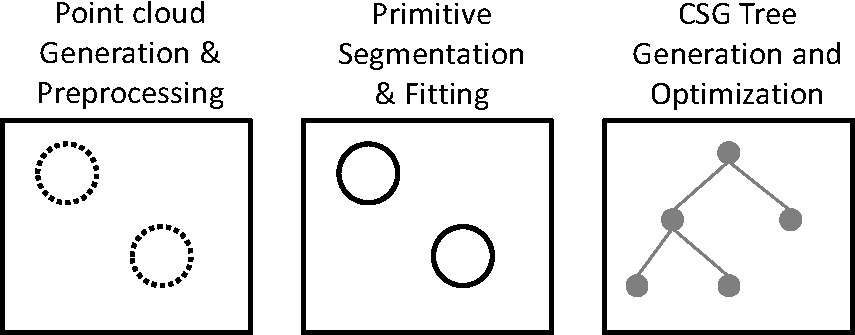
\includegraphics[width=0.5\textwidth]{figures/Praesentation1.pdf}
	\caption{Insert caption to place caption below figure.}
	\label{fig:spp}
\end{figure}

\subsection{Boolean Set-Operations}
The set-operations intersection, union, complement and subtraction are implemented using $\min-$ and $\max$-functions \cite{ricci197constgeo}: 
\begin{itemize}
	\item Intersection: $\cap(S_1,S_2) := \min(f_{S_1}, f_{S_2})$
	\item Union: $\cup(S_1,S_2) := \max(f_{S_1}, f_{S_2})$
	\item Complement: $\not \enskip(S) := -f_S$
	\item Subtraction: $\setminus(S_1,S_2) := \cap(\not \enskip(S_1), S_2)$% = max(-f_{S_1}, f_{S_2})$
\end{itemize}
In the following, the considered boolean set-operations are $\{\text{intersection}, \text{union}, \text{subtraction}\}$.
\subsection{Evolutionary Algorithms} 
TODO: Short description maybe with pseudo code.
\\
%%%%%%%%%%%%%%%%%%%%
%%% Related Work %%%
%%%%%%%%%%%%%%%%%%%%
\section{Related Work}
The problem under consideration is related to the problem of boundary representation (B-Rep) 
to CSG conversion. 
It was first investigated in two-dimensional space for linear polygons, then 
later extended by Shapiro for handling curved polygons \cite{shapiro1991efficient, shapiro2001convex}. 
The extension to three-dimensional objects was initially solved 
by Shapiro and Vossler in \cite{shapiro1991construction, shapiro1993separation}. 
An improved algorithm was later proposed by 
Buchele and Crawford in \cite{buchele2004three}. 
These methods rely on the fact that surfaces are composed of quadric surface patches 
(for computing separators, for factoring dominating halfspaces). 
The algorithm described in \cite{shapiro1991construction} has exponential time complexity.
% I don't understand what the complexity of shapiro1993separation is? 
The algorithm described in \cite{buchele2004three} has cubic (in the number of primitives) time complexity, however the authors remark that the worst time complexity could be exponential. 
\\
Another issue of these approaches is the handling of inexact representations. 
The methods work under the assumption that the patches form a clean partition of the 
target solid. However, in practice we are dealing with input point-clouds that are potentially 
noisy, contain holes, or have additional details and thus the fitted primitives may not fit perfectly. 
This would impact the cellular classification on which the methods described in \cite{shapiro1991construction, shapiro1993separation, buchele2004three} rely. 

%%%%%%%%%%%%%%%%%%%%%%%%%
%%% Problem Statement %%%
%%%%%%%%%%%%%%%%%%%%%%%%%
\section{Problem Statement}
The problem of accelerating \ac{GA}-based \ac{CSG}-tree extraction from point clouds is considered as the open research question addressed by this paper.
\\
As input, a point-set of potentially noisy $3$-d measurements of a connected geometric model together with segmented and fitted primitives is considered. 
The point-set might contain outliers and incomplete regions due to measurement errors that affect the result quality of the primitive reconstruction step.
\\
The desired output is a \ac{CSG}-tree that represents the scanned real-world model as accurately as possible.
\ac{CSG}-tree extraction approaches based on a \ac{GA} \cite{fayolle2016evolutionary} can handle the aforementioned inaccuracies but come with the disadvantage of high computation times.
%With each point, a position $p$ and its estimated normal vector $n$ is stored.  
%There is no further topological information given. 
%- Fehlerbehaftete und fehlende Punktwolken
%- CSG erstellen

%%%%%%%%%%%%%%%
%%% Concept %%%
%%%%%%%%%%%%%%%
\section{Concept}
The basic idea for \ac{GA} acceleration is to partition the search space in independent groups of spatially overlapping primitives.
This exploits the fact that primitives that do not overlap are not considered to be operands of a \ac{CSG}-operation.
\ac{CSG}-extraction is then conducted on a per-partition level. 
Finally, resulting trees are combined in a subsequent merge step without loss of result quality. 
\\
An overview of the full \ac{CSG}-extraction pipeline is depicted in Figure \ref{fig:pipeline_s}. 
Each of the following Chapters describes a particular pipeline step in detail, following the order of execution.

\subsection{Primitive Overlap Graph Generation}
\label{ch:pog}
For expressing spatial relationships between primitives, the \ac{PO}-Graph is introduced.
It represents spatial overlap between primitives using an undirected graph $G=(P,O)$, where $P = \{p_1,\dots,p_{n_p}\}$ is the set of $n_p$ primitives as vertices and $O$ is the edge-set that contains $2$-tuples of overlapping primitives $o=(p_i,p_j)$, where $i,j \in \{1,\dots,n_p\} \land i \ne j$. 
\\
The \ac{PO}-Graph is generated based on the location, orientation and geometric shape of the primitives, see Figure \ref{fig:pipe1} for an example.
Complex shapes can be approximated with simpler hull volumina like \acp{AABB} or \acp{OBB}.
\\
For better scaling, computational complexity can be reduced from $\mathcal{O}({n_p}^2)$ (overlap check between each primitive and each other primitive) to $\mathcal{O}(n_p\log(n_p))$ using hierarchical space partitioning schemes like Octrees \cite{meagher1982Octree}.
\subsection{Search Space Partitioning}
With known primitives and their spatial relations given by the \ac{PO}-graph, the goal is now to find independent search space partitions. 
\\
A partition is a set of primitives in which each primitive has an overlap with each other primitive.
In this context, independence means that per-partition solutions are not influenced by the solutions of other partitions.
See Figure \ref{fig:part} for explanatory examples. 
\\
The problem of finding all independent search space partitions is equivalent to the problem of finding all maximum complete subgraphs (maximum cliques) in $G$.
For finding the set of maximal cliques in $G$, the \ac{BKA}\cite{bron1973cliques} is employed due to its behavior on random graphs.
It was shown experimentally \cite{bron1973cliques} that computation times of \ac{BKA} are almost independent on graph size for random graphs.
In a worst case scenario (using Moon-Moser Graphs \cite{moon1965cliques}), computation times are proportional to $(3.14)^{\frac{n}{3}}$, where $n$ is the size of the graph.
\\
Note that, if there is only a single partition for a particular \ac{PO}-graph, the search space partitioning method degenerates to standard \ac{GA}-based \ac{CSG}-tree extraction. 
The number of resulting partitions also depends on the accuracy of the hull approximation used for primitives during \ac{PO}-graph generation: 
The inaccurate the approximation, the less partitions will emerge.

\begin{figure}[htb]
	\centering
	\begin{subfigure}[b]{0.3\linewidth}
		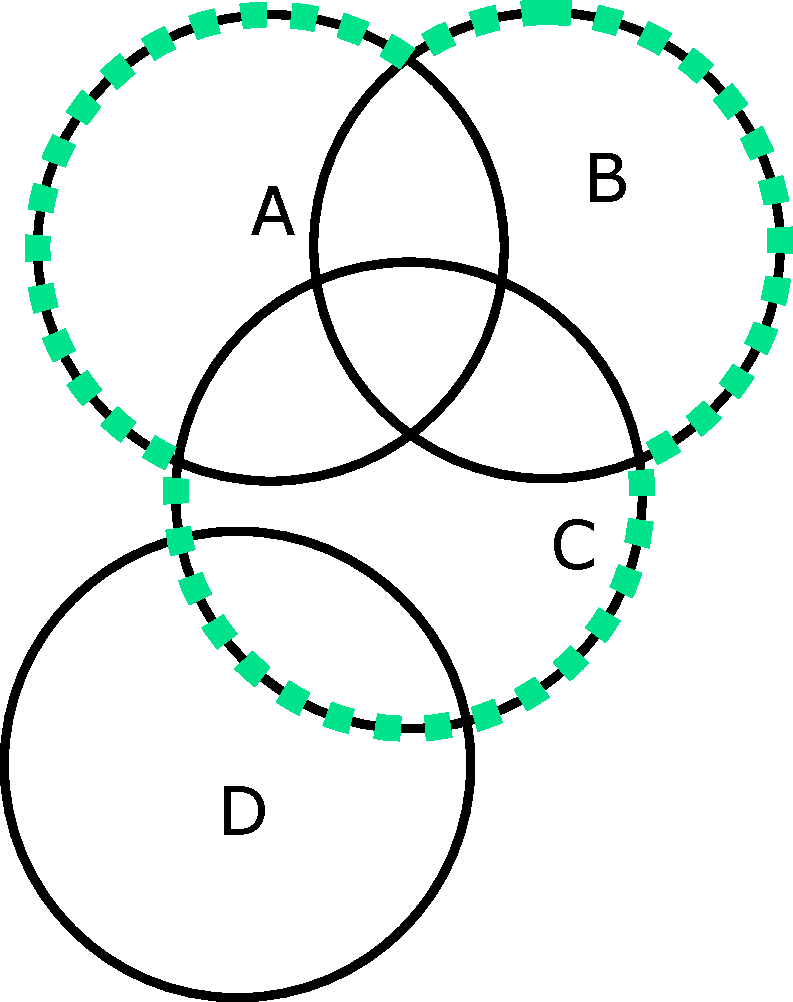
\includegraphics[width=\textwidth]{figures/right_part.pdf}
		\caption{correct}
	\end{subfigure}
	~
	\begin{subfigure}[b]{0.3\linewidth}
		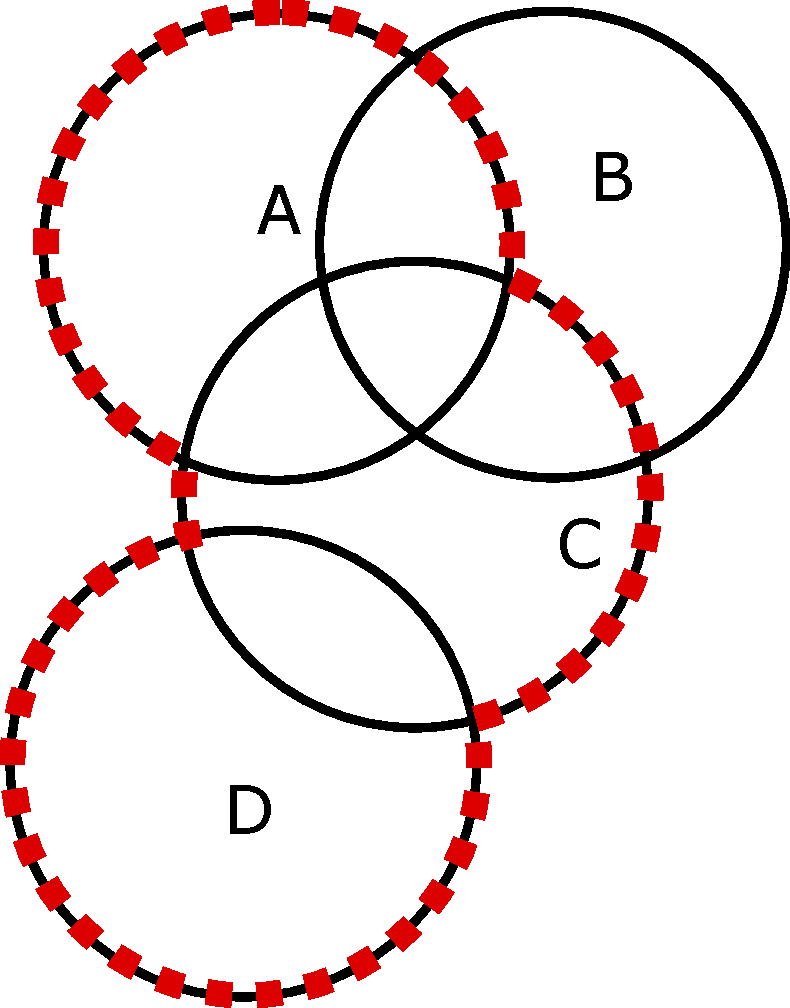
\includegraphics[width=\textwidth]{figures/wrong_part.pdf}	
		\caption{incorrect}
	\end{subfigure}
	\vskip\baselineskip	
	\caption{In the incorrect partition (red), B influences the per-partition solution without being part of the partition.}\label{fig:part}
\end{figure}

\subsection{Per-Partition \ac{CSG}-Tree Extraction}
\label{ch:ga}
With known partitions, \ac{CSG}-tree extraction is conducted for each partition separately in a divide-and-conquer manner.
As basic building block for all acceleration schemes proposed in this paper serves a variant of the \ac{GA} described in \cite{fayolle2016evolutionary} with the objective function
\begin{equation}
\label{eq:of}
E(t, S) := \sum_{i=1}^{|S|}{e^{-d_i(t)^2}+e^{-\theta_i(t)^2}}-\alpha \cdot size(t),
\end{equation}
where $t$ is the tree candidate, $S$ is the point-set and $size(t)$ is the number of nodes in tree $t$ weighted by $\alpha$.
$d_i(t) = \beta \cdot f(s_i)$ is the signed distance between point $s_i$ and the surface defined by tree $t$ weighted by $\beta$.
$\theta_i(t) = \gamma \cdot  \arccos(\nabla \hat{f}(s_i) \cdot n_i)$ is the angle between the point normal $n_i$ and the normalized gradient at position $s_i$ weighted by $\gamma$.  
$\alpha, \beta$ and $\gamma$ are user-controlled parameters. 
The first term in Equation \ref{eq:of} estimates how close the surface induced by $c$ matches the point cloud, the second term penalizes large (in terms of number of nodes) trees.
The third term penalizes large trees.
\\
Initially, the population $T_0$ is filled with $n_T$ randomly generated trees with a height $\le h_{max}$. 
Each \ac{GA} iteration $i$ contains the following steps:
\begin{enumerate}
\item The population of the last iteration $T_{i-1}$ is ranked according to Equation \ref{eq:of}.
\item The current population is initialized with the $n_b$ best candidates from $T_{i-1}$.
\item As long as $T_i$ has not reached maximum population size $n_T$, two crossover candidates were selected from $T_{i-1}$ via Tournament Selection \cite{miller95genetic} parametrized with $k_{ts}$.
During crossover, the two candidates exchange randomly selected subtrees with a probability of $\gamma_{cr}$.
The resulting two trees are then mutated. 
In the mutation process a randomly chosen subtree is replaced with a new randomly generated subtree with a probability of $\gamma_{mu}$.
With a probability of $1-\gamma_{mu}$, the whole tree is replaced with a randomly generated tree.
\item The termination condition is met, if the score of the best \ac{CSG}-tree candidate of an iteration does not improve over $n_{tc}$ iterations.  	 
\end{enumerate}  
The main difference of the described \ac{GA} variant compared to the \ac{GA} proposed in \cite{fayolle2016evolutionary} is the use of truncated solid primitives instead of implicitly defined surfaces of infinite extend in at least one dimension (eg. planes, cylinders). 
This simplifies the algorithm since no additional limiting primitives must be introduced prior to extraction.
\\
The most computational expensive step in \ac{GA}-based \ac{CSG}-tree recovery is the evaluation of Equation \ref{eq:of} for each element of a candidate-set. 
Since evaluations can be conducted for each candidate independently, parallel processing schemes can be efficiently applied.  
In addition, The solution space partitioning allows for an additional per-partition parallelization strategy.
Both options were implemented for multi-core processors and evaluated in Chapter \ref{eq:of}.
\subsection{Merge of Per-Partition Trees}
Merging all trees corresponding to partitions in a single tree is not trivial. 
A simple union of all tree root nodes leads to incorrect results if primitives that are part of multiple cliques are not splitted, see Figure \ref{fig:munion} for an example.
Split operations on arbitrary primitive shapes tend to be complex and thus should be avoided, see e.g. Figure \ref{fig:msplitting}.  
The proposed merge strategy does not need splits but instead tries to merge trees that have a common subtree.
It consists of the following steps:
\begin{itemize}
	\item All trees are inserted in a list $L_t$. 
	\item Two trees $t_0$ and $t_1$ are removed from the end of $L_t$, and their largest common subtree $t_{lcs}$ is computed. The subtree's leaf-set must be a subset of the leaf-sets of $t_0$ and $t_1$. 
	If $t_{lcs}$ is empty, $t_1$ is inserted at the begin of $L_t$ and a new tree candidate $t_1$ is removed from the end of $L_t$. This step is then repeated.
	\item Each node in $t_{tlc}$ exists twice: Once in $t_0$ and once in $t_1$. 
	For each leaf node in $t_{tlc}$ it is checked if its corresponding node in $t_0$ and $t_1$ is a merge candidate.
	This is done by traversing $t_0$ and $t_1$ from root to leaves following Algorithm \ref{al:trav}.
	If the node is reached that way, it is a valid candidate in $t_0$ or $t_1$. 
	Once a valid merge node candidate is found in one tree, it is replaced by the root of the other tree resulting in a merged tree $t_m$.
	If the merge node candidate is valid in both trees, the candidate of the larger tree is replaced by the root of the smaller tree. 
	\item $t_m$ is inserted at the end of $L_t$.
	\item The merge process is continued until there is only a single node left in $L_t$.
	Since the model to reconstruct is by definition connected, the merge process always terminates.
\end{itemize}
The merge process has an asymptotic computational complexity of $\mathcal{O}(\vert L_t \vert^2)$ since in worst case $L_t$ has to be completely traversed for each merge.
Note that the proposed algorithm does not guarantee to find the $t_m$ with the minimal number of nodes possible. 

\begin{algorithm}[htb]
\SetKwProg{myproc}{Procedure}{}{}
\SetKwFunction{proc}{isValid}
\myproc{\proc{curNode, node}}{
	\uIf{curNode = node}{
		\KwRet {true}
	}
	\uIf{curNode.nodeType = Operation}{
		\uIf{curNode.operationType = Difference}{
			\KwRet {\proc{curNode.childs[0]}}
		}
		\uElseIf{curNode.operationType = Union}{
			\ForEach{child $\in$ curNode.childs}{
				\uIf{\proc{child}}{
					\KwRet {true}
				}
			}
		}	 	
	}	
	\KwRet {false}
}

\nl	\proc{$t$.root, node}
\caption{Checks if node \textit{node} is a valid merge candidate in tree $t$.}\label{al:trav}
\end{algorithm}

\begin{figure}[htb]
	\centering
	\begin{subfigure}[b]{\linewidth}
  		\centering
		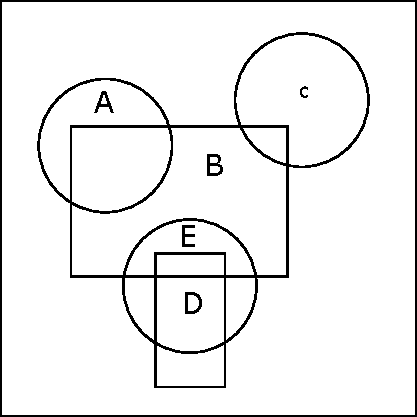
\includegraphics[width=0.3\linewidth]{figures/wm_0.pdf}
		\hfill
		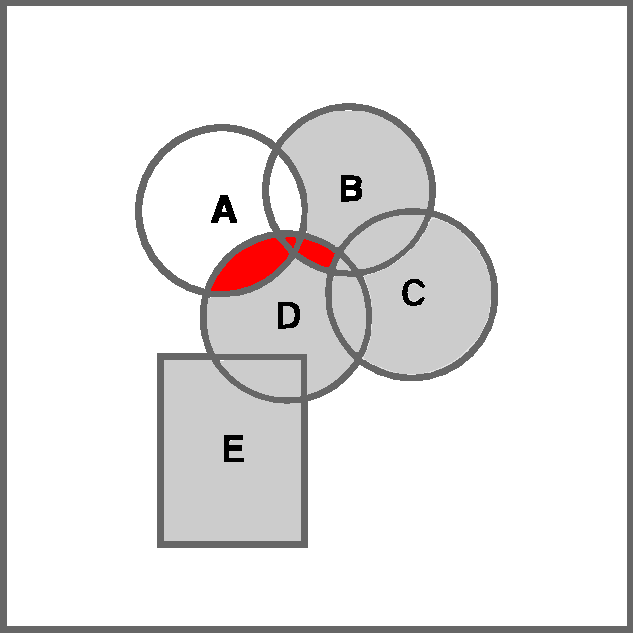
\includegraphics[width=0.3\linewidth]{figures/wm_1.pdf}
		\hfill
		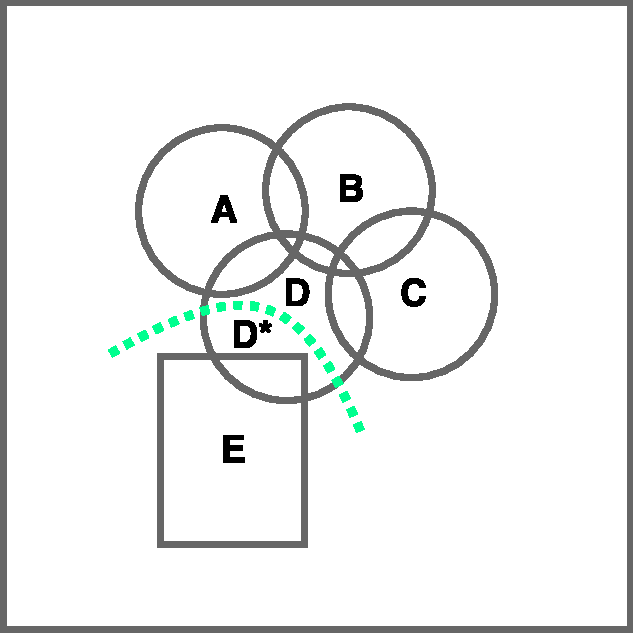
\includegraphics[width=0.3\linewidth]{figures/wm_2.pdf}		
		\caption{Simple tree merge using union over all clique trees. Erroneous geometry in red.}
		\label{fig:munion}
	\end{subfigure}
	\vskip\baselineskip
	\begin{subfigure}[b]{\linewidth}
		\centering
		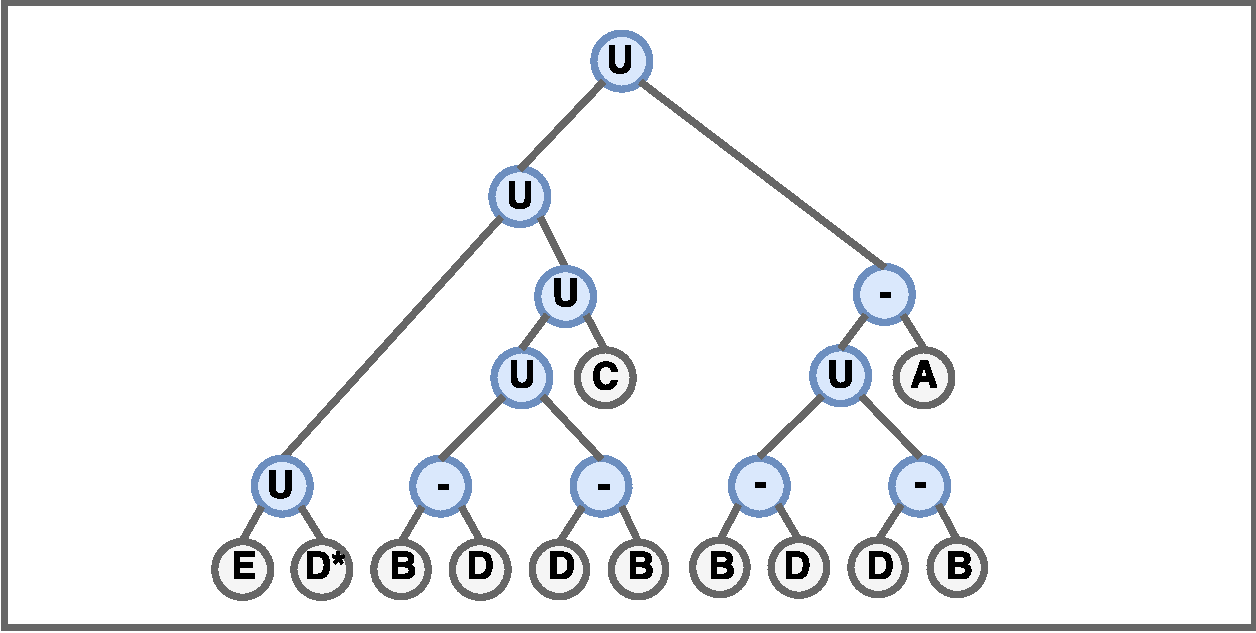
\includegraphics[width=0.3\linewidth]{figures/wm_3.pdf}
		\hfill
		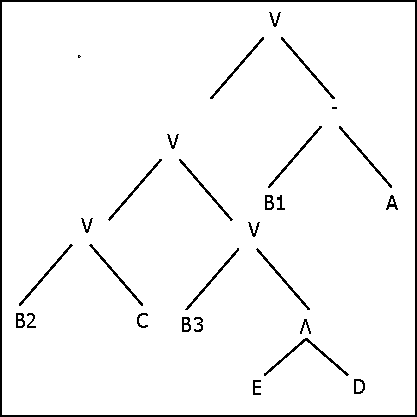
\includegraphics[width=0.3\linewidth]{figures/wm_4.pdf}
		\hfill
		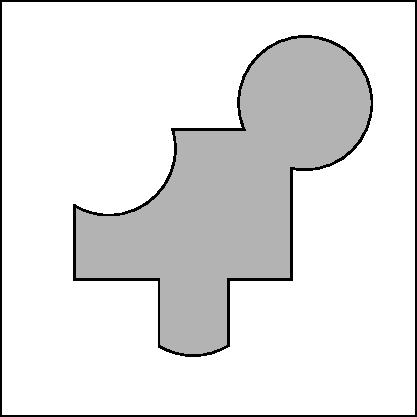
\includegraphics[width=0.3\linewidth]{figures/wm_5.pdf}		
		\caption{Tree merge using primitive splitting.}
		\label{fig:msplitting}
	\end{subfigure}
	\vskip\baselineskip
	\caption{Merge strategies.}\label{fig:wmerge}
\end{figure}

\begin{figure}[htb]
	\centering
	\begin{subfigure}[b]{0.3\linewidth}
		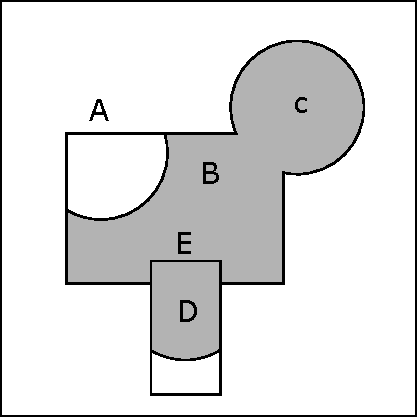
\includegraphics[width=\textwidth]{figures/pipe_0.pdf}
		\caption{Primitives.}
		\label{fig:pipe0}
	\end{subfigure}
	~
	\begin{subfigure}[b]{0.3\linewidth}
		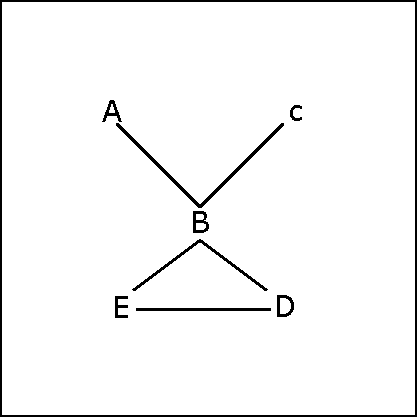
\includegraphics[width=\textwidth]{figures/pipe_1.pdf}
		\caption{\ac{PO}-graph.}
		\label{fig:pipe1}
	\end{subfigure}
	~
	\begin{subfigure}[b]{0.30\linewidth}
		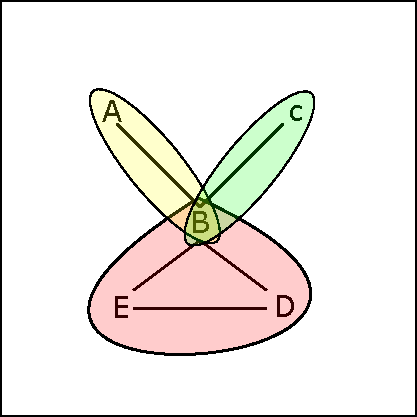
\includegraphics[width=\textwidth]{figures/pipe_2.pdf}
		\caption{Cliques.}
		\label{fig:pipe2}
	\end{subfigure}
	\vskip\baselineskip
	\begin{subfigure}[b]{0.633333\linewidth}
		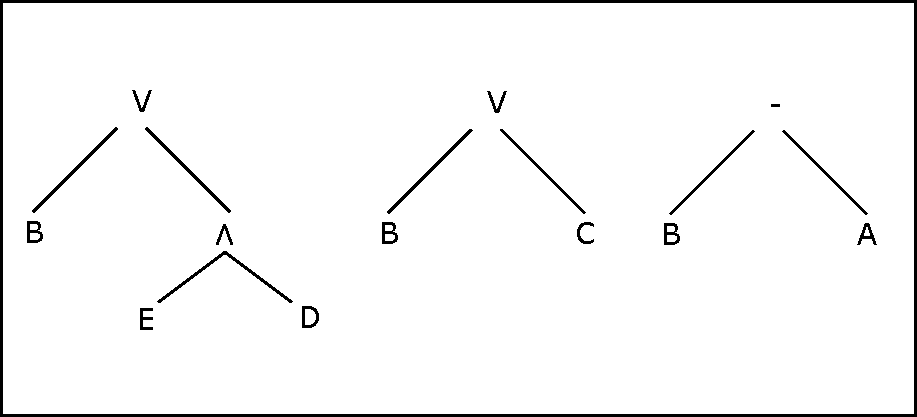
\includegraphics[width=\textwidth]{figures/pipe_4.pdf}
		\caption{Per-clique trees.}
		\label{fig:pipe3}
	\end{subfigure}
	~
	\begin{subfigure}[b]{0.30\linewidth}
		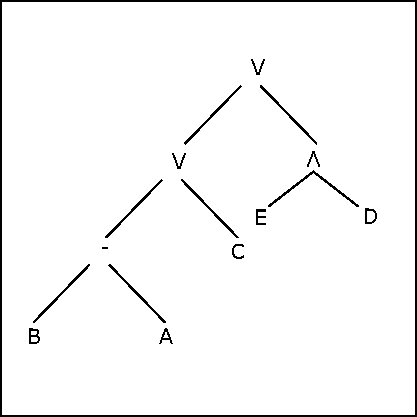
\includegraphics[width=\textwidth]{figures/pipe_3.pdf}
		\caption{Merged tree.}
		\label{fig:pipe4}
	\end{subfigure}
	\vskip\baselineskip	
	\caption{The search space partitioning pipeline.}\label{fig:pipeline_s}
\end{figure}



%%%%%%%%%%%%%%%%%%
%%% Evaluation %%%
%%%%%%%%%%%%%%%%%%
\section{Evaluation}
\label{ch:eval}
The proposed partitioning scheme was evaluated on a laptop with quad core CPU and $16$GB of RAM.
Point-clouds were generated by sampling a model surface induced by a pre-defined \ac{CSG}-tree that served as ground-truth. Gaussian noise was added to sampling points to simulate measurement errors.
\\
Two models were used with different point sampling rates, see Table \ref{tab::models} for details. 
\begin{table}[h]
	\centering
	\begin{tabular}{|l|l|l|l|l|l|}
	\hline
	 & \textbf{M0} & \textbf{M1} & \textbf{M2} \\
	\hline
	\# Primitives & 17 & 4 & 29 \\
	\hline
	\# Points (low) & 11.3k & 9.3k & 10.9k\\
	\hline
	\# Points (high) & 156.4k & 158.4k & 155.4k\\
	\hline
	\# Partitions & (0,8,4,0,1,1) & (0,0,2) &  (0,0,0,12)\\
	\hline	
	\end{tabular}
	\caption{Details on evaluated models. 'low' and 'high' indicate different sampling rates. Numbers of partitions are depicted per partition size. First position in parantheses indicate number of partitions of size $1$ and so on.}
	\label{tab::models}
\end{table}
Baseline is the \ac{GA} approach proposed in \cite{fayolle2016evolutionary} and described in Chapter \ref{ch:ga} The parameter set used for both, baseline and partitioning scheme, is listed in Table \ref{tab:gaparams}.
\begin{table}[h]
	\centering
	\begin{tabular}{|l|l|}
		\hline
		\textbf{Parameter Name} & \textbf{Value}  \\
		\hline
		Population size $n_T$ & 150 \\
		\hline
		\# Best parents $n_b$ & 2 \\
		\hline
		Crossover probability $\mu_{cr}$& 0.3 \\
		\hline
		Mutation probability $\mu_{mu}$& 0.3 \\
		\hline
		Tournament selection parameter $k_{ts}$ & 2\\
		\hline
		Tree size weight $\alpha$& $\log(\text{\#points})$\\
		\hline
		Distance weight $\beta$& $100.0$ \\
		\hline
		Angle weight $\gamma$& $18.0/\pi$ \\
		\hline 
		\# Iterations w/o quality increase $n_{tc}$ & 10 \\
		\hline 
		Maximum tree height $h_{max}$ & $\sqrt{\pi\cdot \vert O \vert}$ \\
		\hline 
	\end{tabular}
	\caption{Parameters for the baseline and search space partitioning approach.}
	\label{tab:gaparams}
\end{table}
The following combinations were evaluated:
\begin{itemize}
	\item Baseline: Single-threaded (BST), multi-threaded \ac{GA} (BMTGA).
	\item Search Space Partitioning: Single-threaded (SST), per-partition multi-threaded (SMTP) multi-threaded \ac{GA} (SMTGA), per-partition and \ac{GA} multi-threaded (SMTPGA).
\end{itemize}     
Timings for baseline and search space partitioning variants were measured for all models with high-detail sampling.
Measurements vary significantly for the same benchmark setting due to the inherently indeterministic behavior of \ac{GA}-based methods. 
In order to deal with the high variance, each experiment was repeated $5$ times.
For model $0$, SMTGA is the fastest method. 
It outperforms baseline by a factor of $15.3$ (single-threaded) and $7.5$ (multi-threaded) on average.
For model $1$, search space partitioning performs worse than baseline: 
The fastest baseline method (BMTGA) is $42.9\%$ slower on average than the best-performing search space partitioning variant (SMTGA).
This can be explained by the relatively small number of primitives in model $1$ which eliminates the need for partitioning.
\\
TODO: Add discussion for model 2.
\\
Search space partitioning with \ac{GA} parallelization (SMTGA) is in general faster than their per-partition counterparts (SMTP, SMTPGA) for all models.
This is due to the granularity and regularity of the parallelization: 
For SMTGA, the task of ranking a population can be splitted in $n_T$ parts, with each part having similar execution times.
For per-partition variants, granularity is determined by the (potentially lower) number of partitions and per-partition execution times may vary a lot dependent on partition sizes. 
\\
See Figure \ref{fig:graph1} for an overview of the results of the complete performance experiment.
Results for per-partition variants do not show timings for different pipeline steps since in all experiments, per-partition \ac{CSG}-tree extraction is by far the most dominant factor. 
The summarized time measures for \ac{PO}-tree generation, search space partitioning and tree merge make less then $1\permil$ of the total runtime.
\\
Figure \ref{fig:graph2} contains average depths and sizes of resulting trees for baseline and partitioning variants.
For the latter, tree depths have increased by $50$-$155\%$ compared to the input tree, while for baseline approaches, an increase of only $0$-$80\%$ is visible.
Tree sizes show similar behavior:
Partitioning variants produce $57$-$77\%$ larger trees, while baseline approaches increase tree size by only $0$-$6\%$.
This adverse behavior of partitioning variants is due to the final merge step:
In each merge iteration, not those two trees with the largest common subtree of all trees in the merge list are merged but those that are neighbors in the merge list and have a common subtree of at least size $1$.
Since focus is on performance, this is acceptable behavior.
\\
Figure \ref{fig:graph3} depicts measurement results for the ratio
\begin{equation} \label{eq:ratio}
\frac{\#\text{points}_{high}}{\#\text{points}_{low}} : \frac{\text{duration}_{high}}{\text{duration}_{low}}
\end{equation}
which quantifies the dependency between point cloud size and corresponding computation times.
It indicates that, for larger models (model $0$ and $2$), the fastest partitioning approach scales up to $1.9$-times better than the best performing baseline approach with respect to point cloud size.
\begin{figure}[htb]
	\centering
	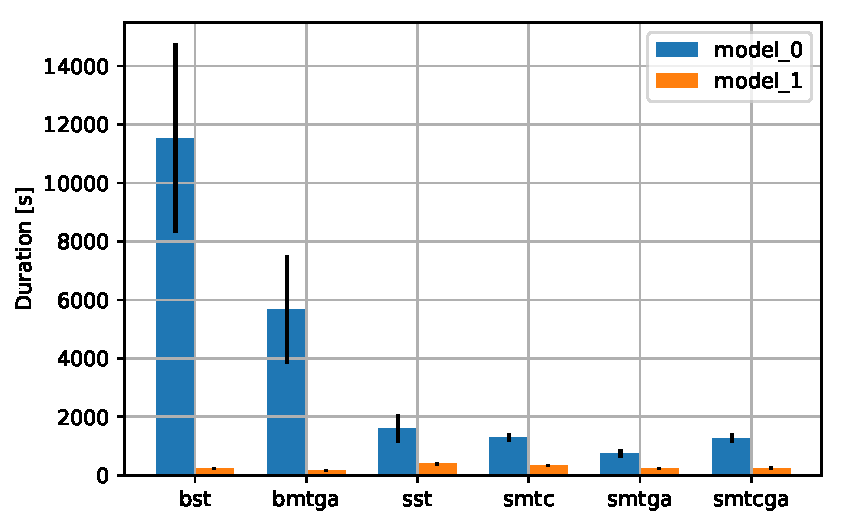
\includegraphics[width=0.5\textwidth]{figures/g1.pdf}
	\caption{Timings for all approach combinations for and models with high-detailed sampling. Vertical black lines indicate standard deviation.}
	\label{fig:graph1}
\end{figure}
\begin{figure}[htb]
	\centering
	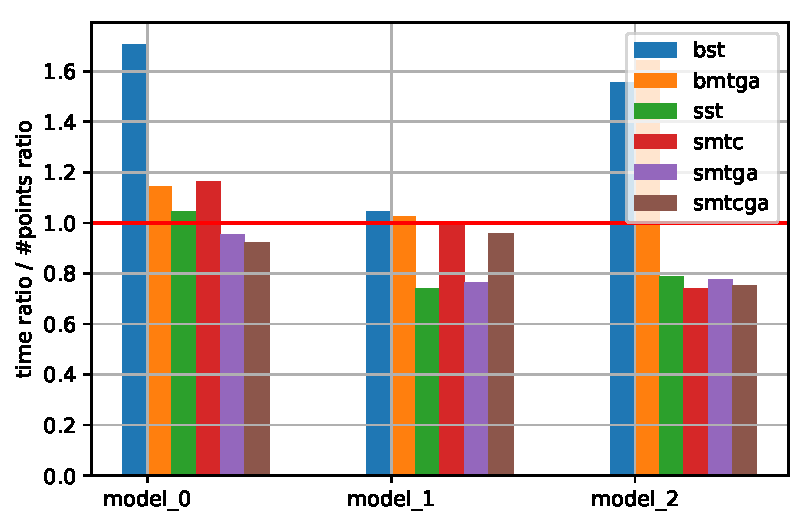
\includegraphics[width=0.5\textwidth]{figures/g3.pdf}
	\caption{Ratio between high-detail and low-detail point cloud size factor and corresponding timing factors for all models (see Equation \ref{eq:ratio}). The red line indicates linear scaling with a slope of $1$ with respect to point cloud size.}
	\label{fig:graph3}
\end{figure}

\begin{figure}[htb]
	\centering
	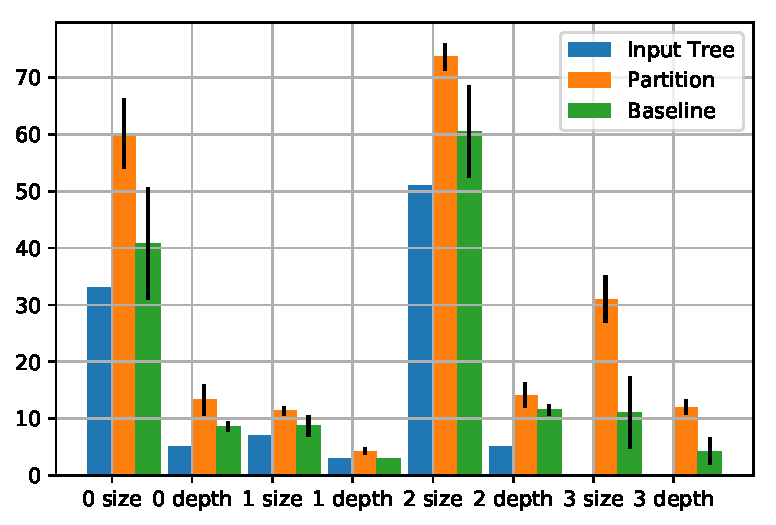
\includegraphics[width=0.5\textwidth]{figures/g2.pdf}
	\caption{Average tree size and depth for baseline and search space partitioning methods for all models with high-detail sampling. Vertical black lines indicate standard deviation.}
	\label{fig:graph2}
\end{figure}
%%%%%%%%%%%%%%%%%%
%%% Conclusion %%%
%%%%%%%%%%%%%%%%%%
\section{Conclusion}
TODO: Summary
\\
The used \ac{GA} might be implement for massively parallel computing hardware and combined with the proposed partitioning approach. 
In addition, point cloud filtering based on sharp feature detection \cite{weber2010sharp} could further increase performance.
A decreased tree size in the partitioning approach could be achieved by improving the merge process.


% XXXXXXXXXXXXXXXXXXXXXXXXXXXXXXXXXXXXXXXXXXX
% XXXXXXXXXXXXXXXXXXXXXXXXXXXXXXXXXXXXXXXXXXX
% XXXXXXXXXXXXXXXXXXXXXXXXXXXXXXXXXXXXXXXXXXX

\section{Acknowledgments}



%-------------------------------------------------------------------------
% example of algorithm typesetting
% to allow this, uncomment line 
% \RequirePackage[noend]{myalgorithm}
% in the wscg.sty file
% and download that package from Gabriel Zachmann's page http://zach.in.tu-clausthal.de/latex/
%
%


%%%%%%%%%%%%%%%%%%%%%%%%%%%%%%%%%%%%%%%%%%%%%%%%%%%%%%%%%%%%%%%%%%%%%%%%%%%%%
\bibliographystyle{alpha} % SFELD
\bibliography{main} % SFELD
\end{document}

